\documentclass[article,12pt,onesidea,4paper,english,brazil,]{abntex2}

\usepackage{lmodern, indentfirst, nomencl, color, graphicx, microtype, lipsum, textcomp}			
\usepackage[T1]{fontenc}		
\usepackage[utf8]{inputenc}		

\setlrmarginsandblock{2cm}{2cm}{*}
\setulmarginsandblock{2cm}{2cm}{*}
\checkandfixthelayout

\setlength{\parindent}{1.3cm}
\setlength{\parskip}{0.2cm}

\SingleSpacing

\begin{document}
	
	\selectlanguage{brazil}
	
	\frenchspacing 
	
	\begin{center}
		\LARGE ATIVIDADES FÍSICAS HABITUAIS DE ALUNOS DO ENSINO BÁSICO, TÉCNICO E TECNOLÓGICO\footnote{Trabalho realizado dentro da área de conhecimento Ciências da Saúde, financiado pela Fundação Rondônia de Amparo ao Desenvolvimento das Ações Científicas e Tecnológicas e à Pesquisa do Estado de Rondônia (FAPERO) e pelo Conselho Nacional de Desenvolvimento Científico e Tecnológico (CNPq).}
		
		\normalsize
	Nícolas Costa Freitas \footnote{Aluno do Curso Técnico em Informática Integrado ao Ensino Médio, nicolasfreitas.0300@gmail.com, Campus Porto Velho Calama.} 
		Iranira Geminiano de Melo \footnote{Orientadora, iranira.melo@ifro.edu.br, Campus Porto Velho Calama} 
	George Madson Dias Santos \footnote{Co-orientador, george.santos@ifro.edu.br, Campus Porto Velho Calama} 
		 
	\end{center}
	
	% resumo em português
	\begin{resumoumacoluna}
		A prática de atividades físicas é importante para o bem-estar do indivíduo, contribuindo com a prevenção de doenças crônico-degenerativas. A prática de atividades físicas deve se tornar algo habitual na vida de qualquer indivíduo, devido aos benefícios que ela traz tanto para a saúde e bem-estar, como na vida social e laboral. Relacionado a isso, esse artigo tem como objetivo informatizar um questionário para avaliação das atividades físicas habituais de alunos de curso técnico integrado ao ensino médio, do Campus Porto Velho Calama. Isso se deu com desenvolvimento de um site onde foi hospedado o questionário da pesquisa.
		
		\vspace{\onelineskip}
		
		\noindent
		\textbf{Palavras-chave}: Informatização. Saúde. Bem-estar.
	\end{resumoumacoluna}
	
	\section*{Introdução}
	
A prática de atividades físicas é um componente do estilo de vida importante para o bem-estar do indivíduo, além disso, se destaca como relevante ferramenta na prevenção de doenças crônico-degenerativas, por isso deve compor a rotina diária de qualquer pessoa. Além da prevenção dos agravos à saúde tem-se os benefícios tanto para o bem-estar como na vida social laboral das pessoas (ASSUMPÇÃO, MORAIS \& FONTOURA, 2002; DELLANI et al, 2014; NAHAS, 2013).

Nesse contexto, a pesquisa teve por objetivo informatizar um questionário para avaliação das atividades físicas habituais de alunos de curso técnico integrado ao ensino médio, do Campus Porto Velho Calama. Para isso foi desenvolvido um site, onde um questionário foi codificado, ficando a disposição para ser respondido. Para tornar o questionário disponível na web,e acessível aos alunos,fez-se necessária a hospedagem da página PHP em um servidor WEB permitindo acesso simultâneo de várias pessoas e o conhecimento automático da avaliação realizada.

	
	\section*{Material e Método}
	
Para esse estudo, analisa-se o questionário denominado Atividades Físicas Habituais, descrito por Nahas (2013). Assim, ao responder ao questionário as informações são armazenadas em um banco de dados, possibilitando avaliação e acompanhamento das atividades físicas habituais dos alunos.

Acredita-se que a informatização do questionário para avaliação das atividades físicas habituais contribuirá em dois âmbitos: para o participante da pesquisa quando ele responder ao questionário terá o resultado imediato, a partir dessa avaliação ele poderá ser motivado a se tornar mais ativo; para o pesquisador os dados estarão sendo armazenado simultaneamente, podendo a qualquer momento fazer a compilação e análise dos resultados.

A forma de pontuação é diferente entre as questões, sendo que as questões que são pontuadas são aquelas que o respondente escolha a opção “sim” (cada questão tem a opção de sim ou não). Depois de responder ao questionário, o aluno recebe uma classificação de acordo com a soma das pontuações. Ele pode ser classificado em: inativo (caso faça de 0 a 5 pontos), pouco ativo (6 a 11 pontos), modera mente ativo (12 a 20 pontos) ou muito ativo (21 ou mais pontos).

Com a intensão de garantir a confiança nos dados coletados, ao desenvolver o banco de dados, foram cadastrados os CPFs dos alunos do Instituto Federal de Rondônia, Campus Porto Velho Calama, para assegurar que apenas eles têm acesso ao questionário.

	
	\section*{Resultados e Discussão}
	
	Obteve como resultado o desenvolvimento de um site onde está hospedado o questionário da pesquisa, conforme a imagem abaixo.
	
	\begin{figure}[h]
		\centering
		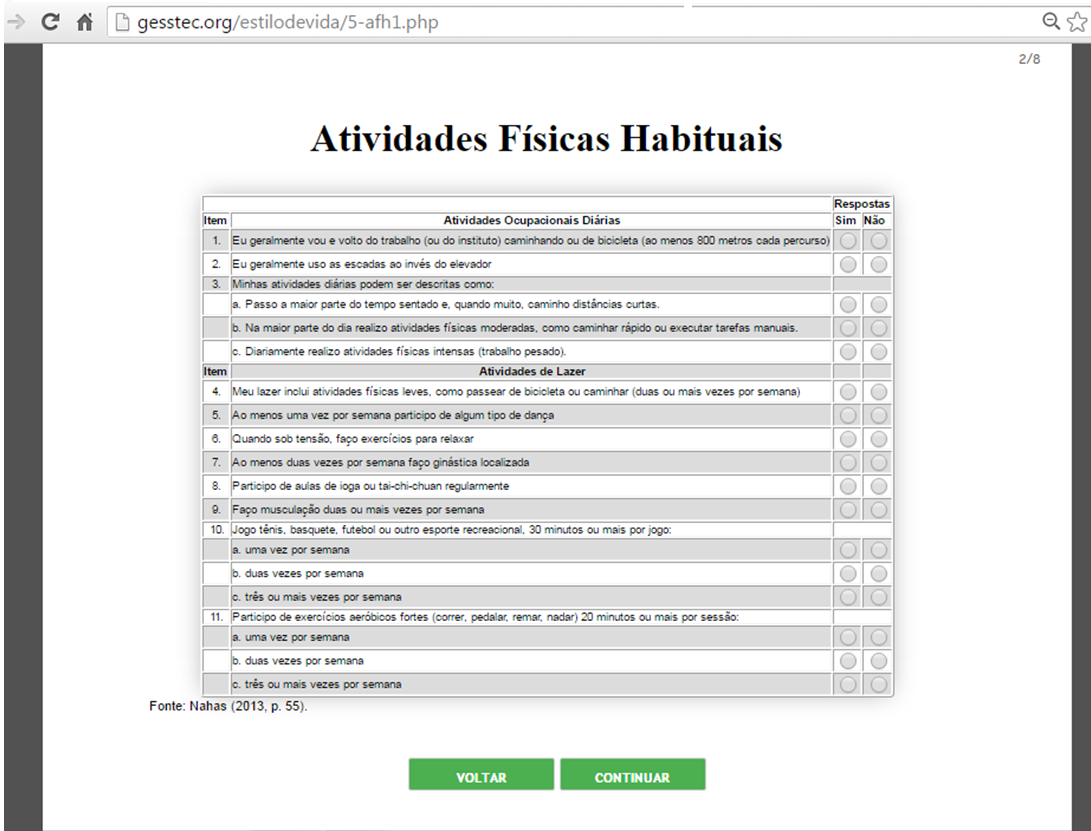
\includegraphics[width=0.7\linewidth]{pip04.png}
		\caption{Ilustração do questionário desenvolvido, Porto Velho, 2016.}
	\end{figure}
Conforme visto, o usuário tem a opção de escolher entre duas alternativas: sim ou não. Após o término do preenchimento do questionário, o usuário irá ser encaminhado para outra página, onde visualizará o resultado, e será classificado em, de acordo com sua pontuação, “efetivo”, “pouco ativo”, “moderadamente ativo” ou “muito ativo”.
O site está disponível no endereço eletrônico: www.gesstec.org/estilodevida/estilodevida.html
	
	\section*{Conclusões}
	
	Com base na realização do projeto de pesquisa, conclui-se que é possível associar informática e educação física para o desenvolvimento de estratégias e de promoção da saúde a partir de ações que contribuam para tornar as pessoas mais ativas fisicamente.
	
	\section*{Instituição de Fomento}
	
	Fundação Rondônia de Amparo ao Desenvolvimento das Ações Científicas e Tecnológicas e à Pesquisa do Estado de Rondônia (FAPERO) e pelo Conselho Nacional de Desenvolvimento Científico e Tecnológico (CNPq).
	
	\sloppy
	\section*{Referências}
	
	\noindent ASSUMPÇÃO, Luís Otávio Teles; MORAIS, Pedro Paulo de; FONTOURA, Humberto. Relação entre atividade física, saúde e qualidade de vida. Revista Digital - Buenos Aires - Año 8 - N° 52 - Septiembre de 2002. Disponível em:
	<http://www.efdeportes.com/efd52/saude.htm>. Acesso em: 30/12/2015.
	
	\noindent DELLANI, Marcos Paulo; BOTTON, Fernanda; COSTA, Gisele Maria Tonin da; MATUSCHAK, Jucilene. Estilo de Vida com Qualidade de Vida: Uma Visão de Complementaridade. Rio de Janeiro: Instituto de Desenvolvimento Educacional do Alto Uruguai – IDEAU, pág. 4, 2014.
	
	\noindent NAHAS, Markus V. Atividade Física, Saúde e Qualidade de Vida. 6 ed. Londrina: Midiograf, 2013.
	
	
\end{document}